\chapter{仿真及飞行试验}
%
本章将展示仿真及飞行试验结果。本文所研究的单涵道风扇式无人机的飞行控制系统的MATLAB$^\circledR$/Simulink$^\circledR$仿真程序已开源,地址:https://github.com/mengchaoheng/Plan-D。该仿真包含利用扩展卡尔曼滤波算法的状态估计,自抗扰控制器以及PID控制器,还包括各类控制分配算法的实现,是本文讨论单涵道部分的内容的基础。由于可以相对独立地进行高度控制,因此本章不考虑高度通道,下述仿真以及飞行试验都是在定高模式下进行。
\section{单涵道仿真分析}
由于实际中无法得到总和扰动的真实值,因此考虑借助所搭建的仿真模型,验证所设计的ESO可实时估计总和扰动。而优先级分配方法的验证,是通过人为构造伪控制指令作为输入再观察输出。
\subsection{模型验证}
所搭建的MATLAB$^\circledR$/Simulink$^\circledR$仿真如图\ref{system}所示的。为考察第二章中所建立的数学模型的准确性,本节将相同输入下,实际飞行试验得到的输出数据与由模型得到的理论值进行对比。在实际飞行操作中,直接通过控制舵面的偏角来控制飞行是十分困难的。考虑到飞行安全,在飞行器$ p$、$q$以及$r$三个通道各串联一PI控制器,使用闭环系统进行仿真和飞行试验。
\begin{figure}[htbp]
	\centering	
	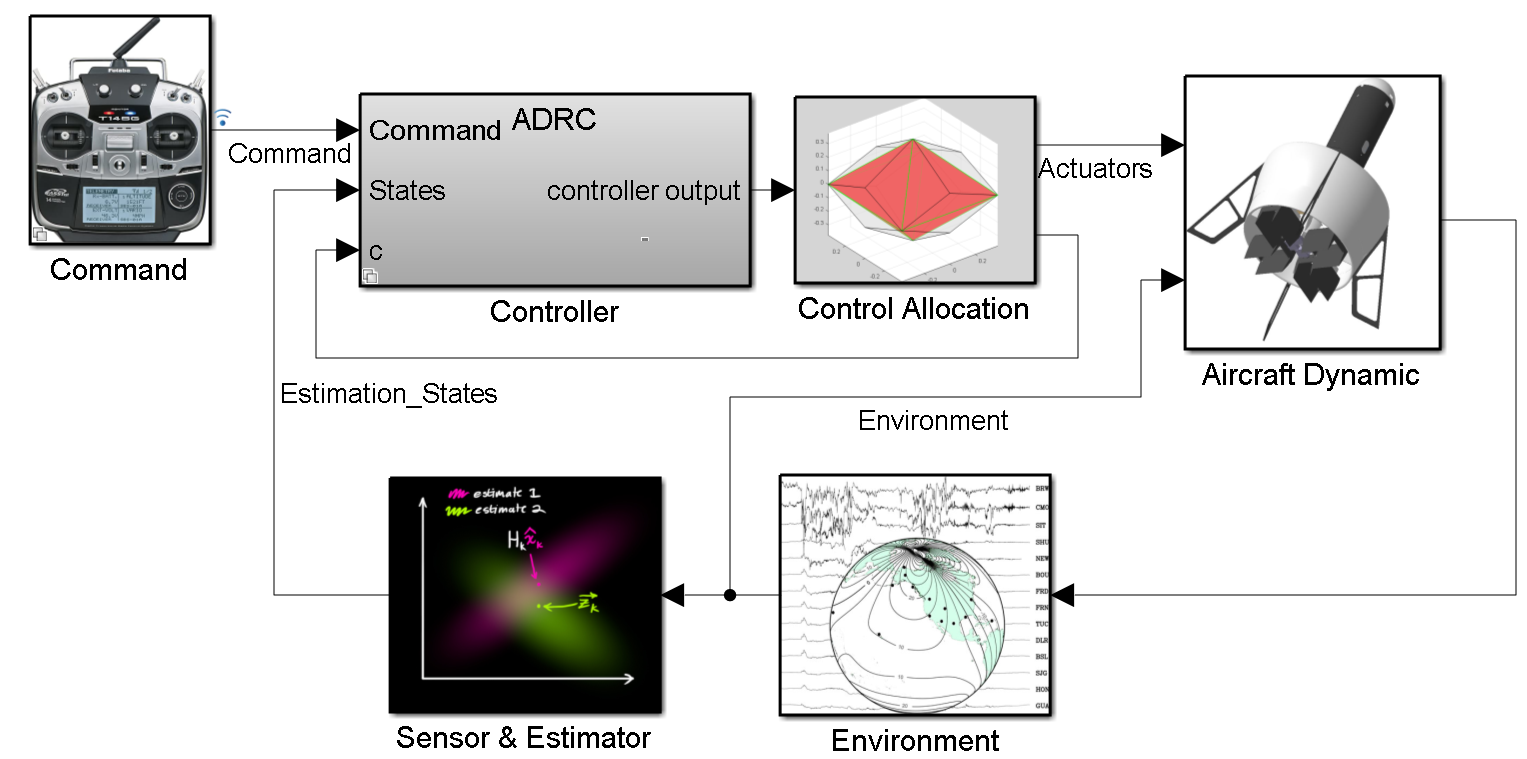
\includegraphics[scale=0.38]{Fig/system.png}
	\caption{\label{system}DFUAV的飞行控制系统}
\end{figure}

在飞行试验时采集输入、输出数据并记录控制器参数。PI控制器设计可参考\cite{Peddle_2009},滚转/俯仰通道比例系数$ k_p=0.5 $、积分系数$ k_i=0.08 $。偏航通道比例系数$ k_p=0.3 $、积分系数$ k_i=0.05 $。将采集到的输入信号作为仿真中的参考输入,仿真输出即理论值。示意图如图\ref{model_and_real}所示。其中$ \bm{\omega}_{ref} $为参考角速度输入。为简单起见,控制分配方法取伪逆法。
\begin{figure}[htbp]
	\centering	
	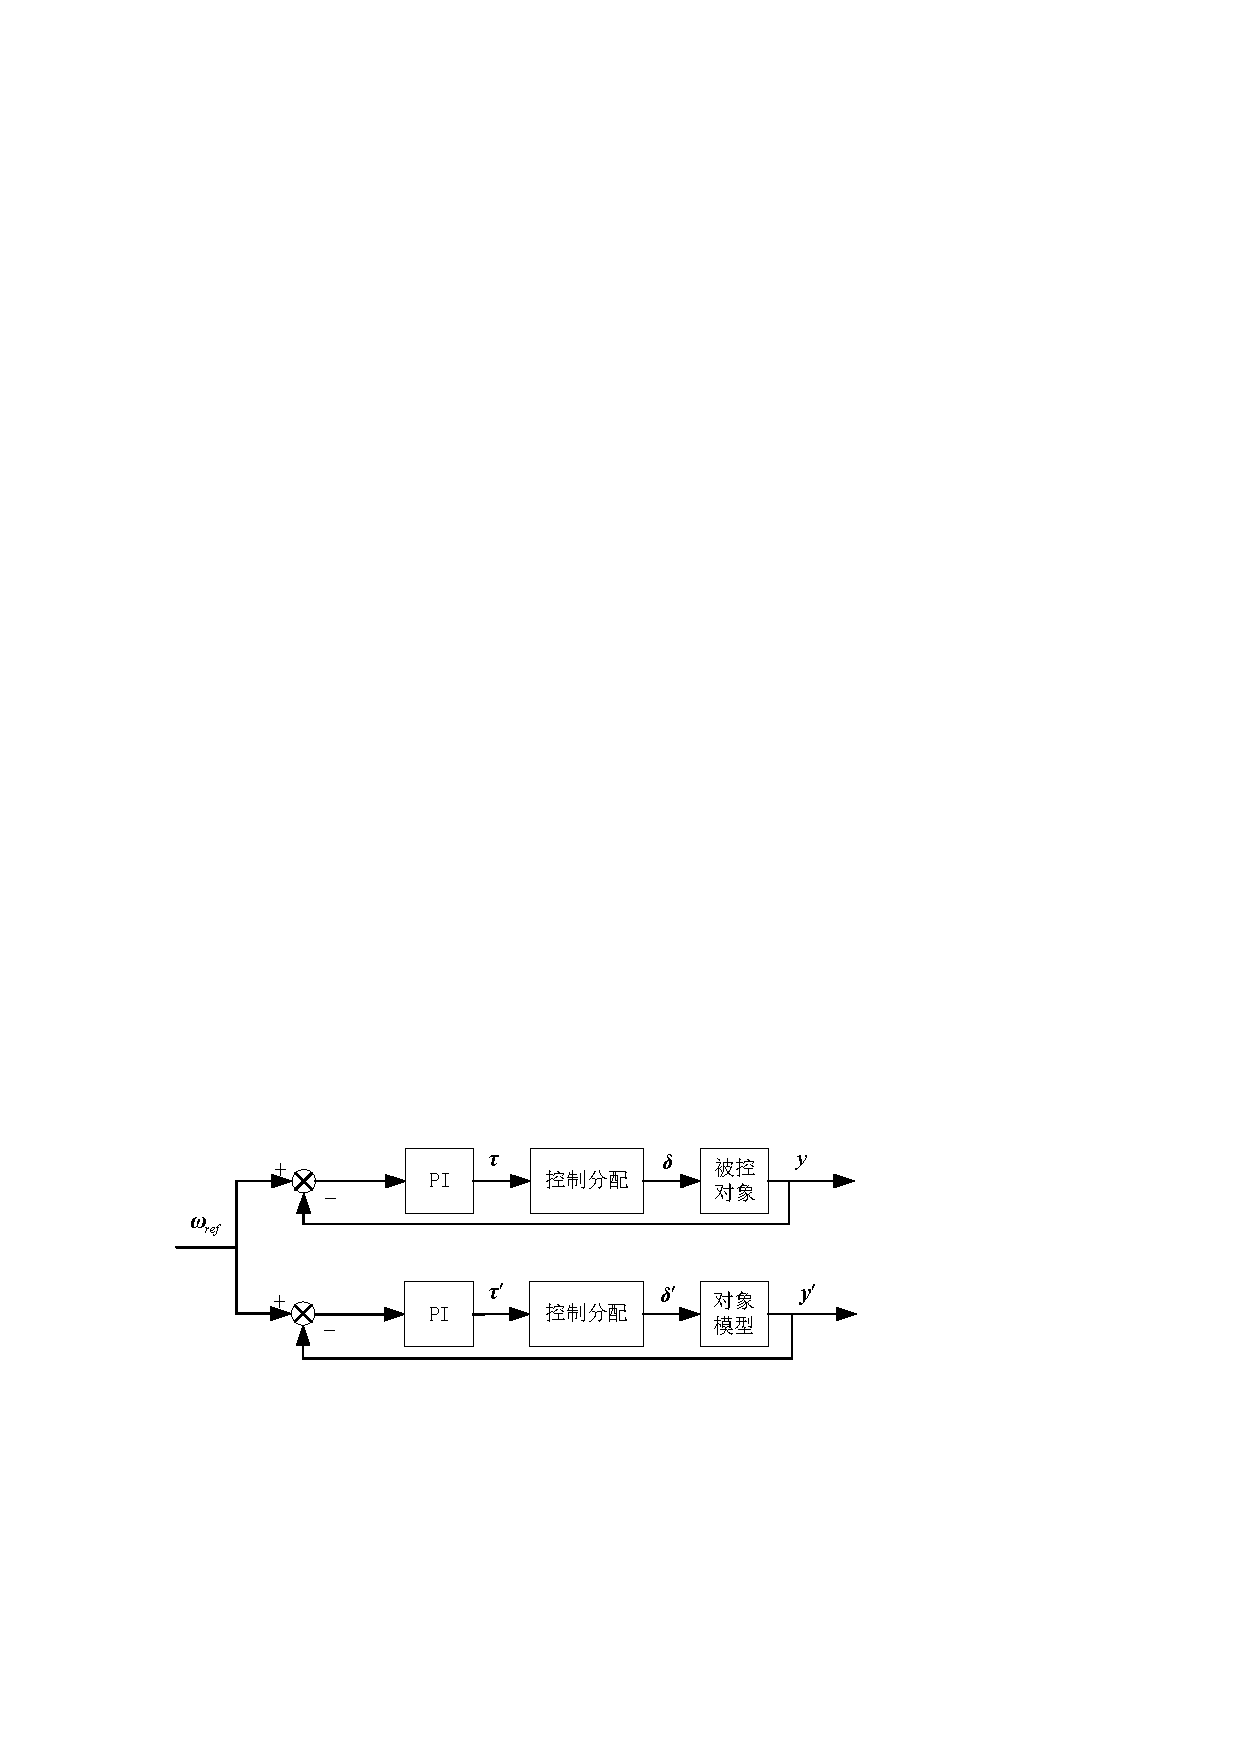
\includegraphics[scale=1]{Fig/model_and_real.pdf}
	\caption{\label{model_and_real}验证方法示意图}
\end{figure}

由于无人机结构对称,因此滚转、俯仰通道的结果是类似的。以滚转为例,在相同参考输入下,仿真得到的滚转角速度$ p $的理论值和飞行试验得到的测量值对比如图\ref{p_m_r}所示,相应通道的滚转角测量值与理论值对比如图\ref{roll_m_r}所示,NED系速度$ V_y $测量值与理论值对比如图\ref{Vy_m_r}所示。
\begin{figure}[htbp]
	\centering	
	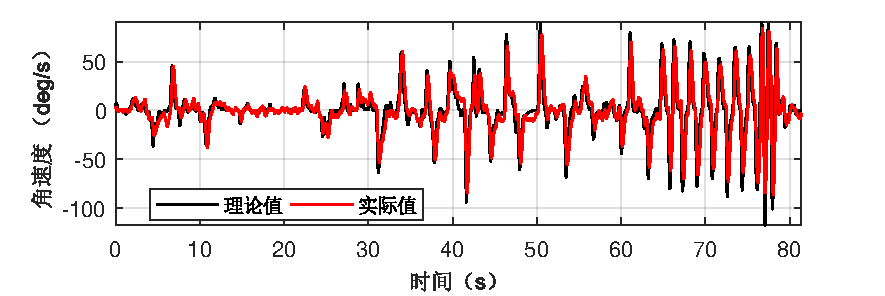
\includegraphics[scale=1]{Fig/p_m_r.pdf}
	\caption{\label{p_m_r}滚转角速度$ p $测量值与理论值}
	%\end{figure}
	%\begin{figure}[htbp]
	\centering	
	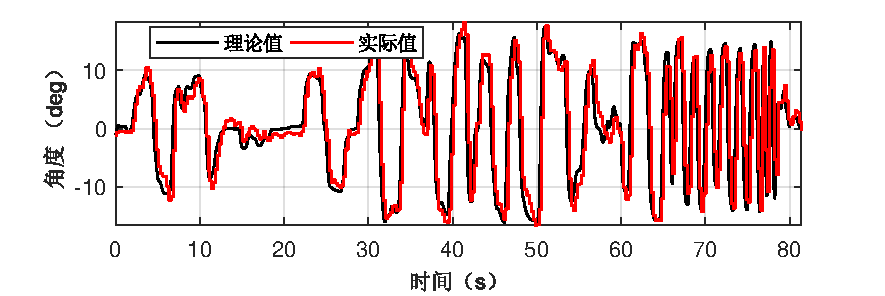
\includegraphics[scale=1]{Fig/roll_m_r.pdf}
	\caption{\label{roll_m_r}滚转角测量值与理论值}
\end{figure}
\begin{figure}[htbp]
	\centering	
	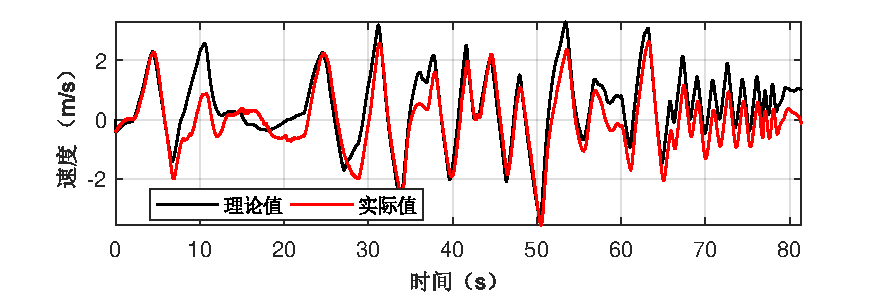
\includegraphics[scale=1]{Fig/Vy_m_r.pdf}
	\caption{\label{Vy_m_r}NED系下速度$ V_y $测量值与理论值}
\end{figure}

偏航通道的验证主要观察偏航角速度与偏航角。偏航角速度$ r $测量值与理论值对比如图\ref{r_m_r}所示。偏航角测量值与理论值对比如图\ref{yaw_m_r}所示。
\begin{figure}[htbp]
	\centering	
	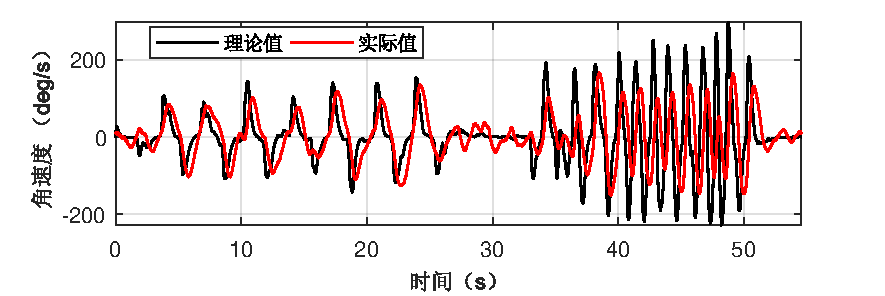
\includegraphics[scale=1]{Fig/r_m_r.pdf}
	\caption{\label{r_m_r}偏航角速度$ r $测量值与理论值}
	%\end{figure}
	%\begin{figure}[htbp]
	\centering	
	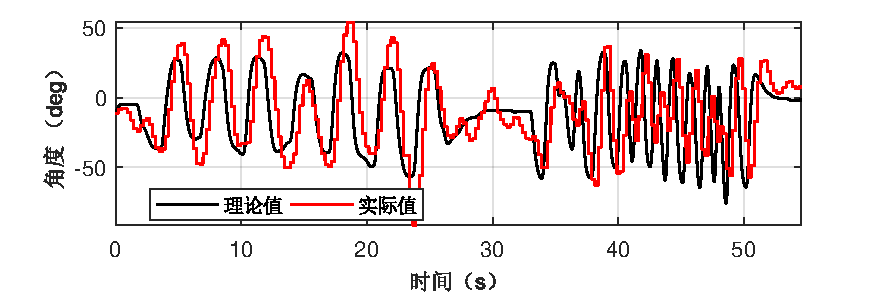
\includegraphics[scale=1]{Fig/yaw_m_r.pdf}
	\caption{\label{yaw_m_r}偏航角测量值与理论值}
\end{figure}
%\begin{figure}[htbp]
%	\centering	
%	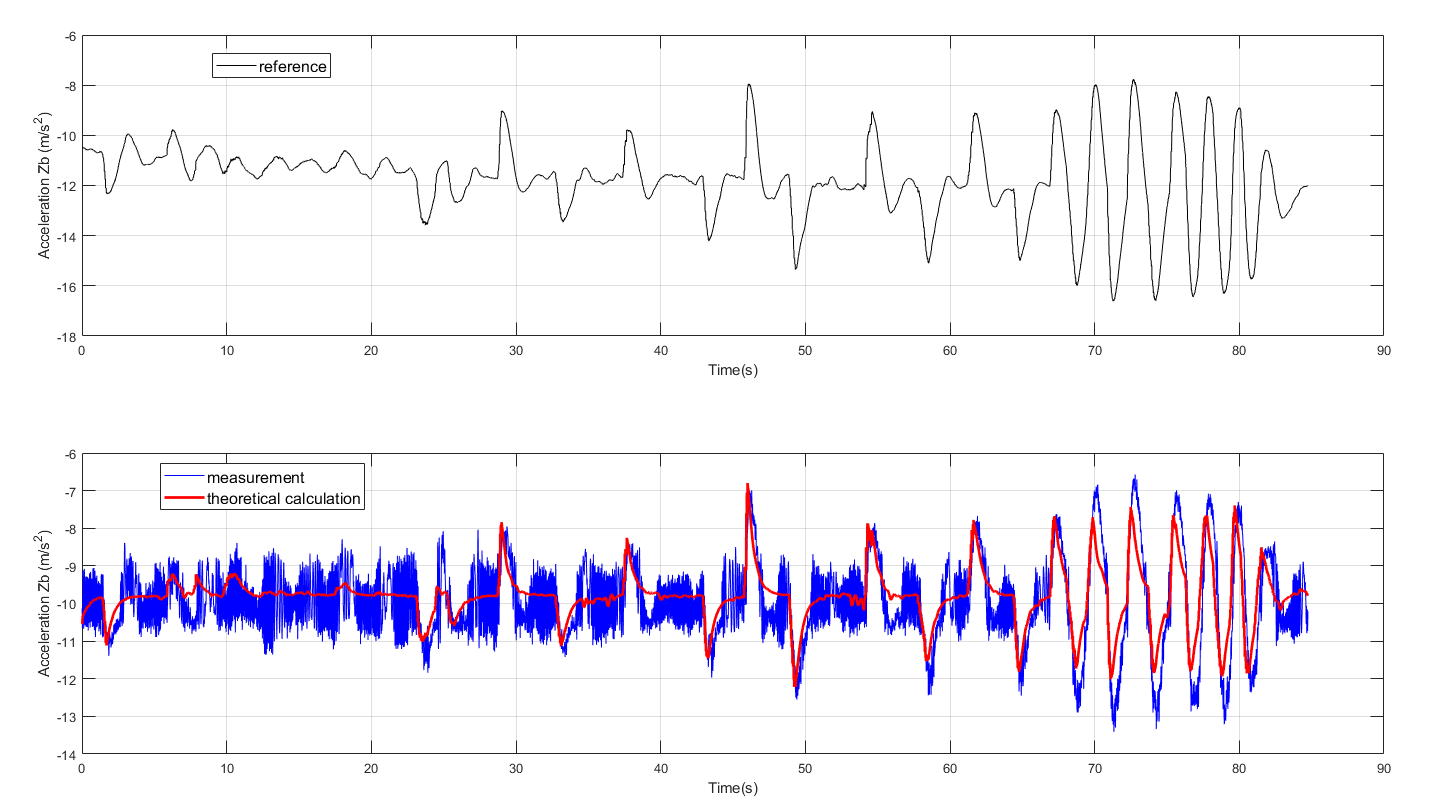
\includegraphics[scale=0.4]{Fig/a_z_m_r.png}
%	\caption{\label{a_z_m_r} $ Z_b $轴方向加速度测量与理论值}
%\end{figure}
%\begin{figure}[htbp]
%	\centering	
%	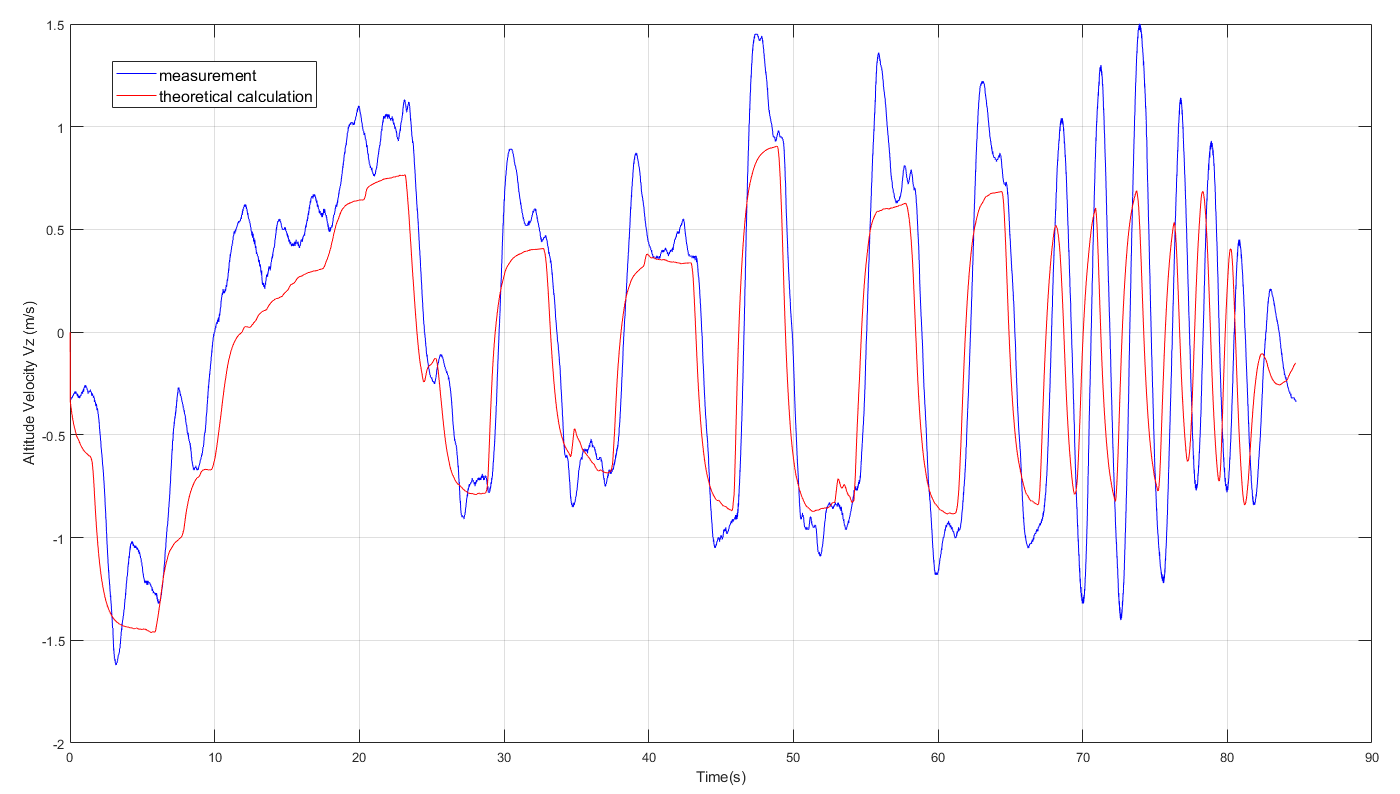
\includegraphics[scale=0.4]{Fig/Vz_m_r.png}
%	\caption{\label{Vz_m_r}地面坐标系下的高度速度$ V_z $的测量与理论}
%\end{figure}
\subsection{ESO仿真}
在定高模式下,使用ADRC控制器进行姿态控制,控制分配方法使用优先级分配法。当俯仰、偏航角参考指令为0,滚转角输入$ \varphi_c $如图\ref{ESO_m_r}中红线所示所示时,总和扰动$ f_1+w_1 $和ESO估计到的扰动$ \hat{x}_3 $对比如图\ref{ESO_m_r}所示。值得注意,同上一小节类似,这里使用何种控制分配方法并不影响结果。
\begin{figure}[htbp]
	\centering	
	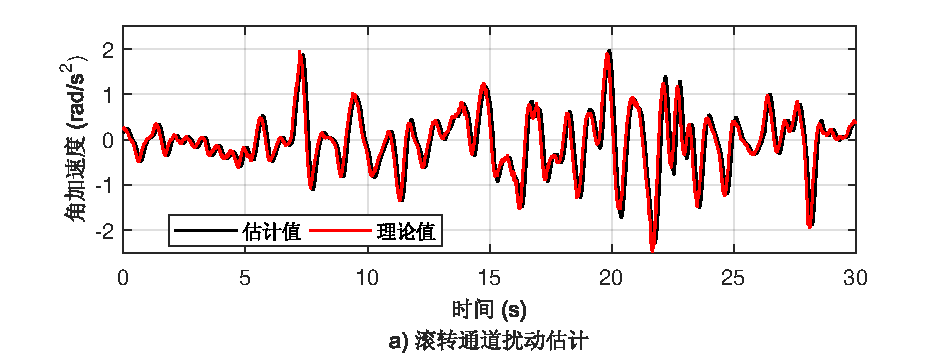
\includegraphics[scale=1]{Fig/ESOa.pdf}
	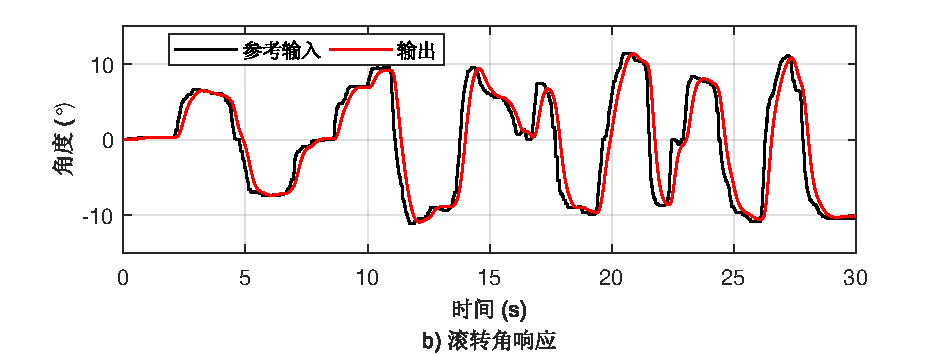
\includegraphics[scale=1]{Fig/ESOb.pdf}
	\caption{\label{ESO_m_r}总和扰动的估计值和理论值对比}
\end{figure}
\subsection{优先级控制分配仿真}
给定期望力矩,使用不同控制分配算法进行仿真。设$ m=3 $ ,$ p=4 $ ,控制效率矩阵 $ \bm{B} $和操纵面约束分别如式\eqref{position_constraints}、式\eqref{control_effectiveness_matrix}所示。并设已按优先级分解的期望力矩为 $\bm{\tau}=\bm{\tau}_1+\bm{\tau}_2$,其中高优先级分量 $\bm{\tau}_1 = [0 \quad 0 \quad 0.25]^\top $、低优先级分量$\bm{\tau}_1 = [0.34\cos(\pi t) \quad 0.34\sin (\pi t) \quad 0.25]^\top $ ,该期望力矩随时间变化,涵盖了可达和不可达的情形。利用simulink的Nonlinear Second-Order Actuator模块作为操纵面执行机构进行仿真。求解控制分配时采用式\eqref{eq_linear_model},速率约束为$400{{}^\circ }/{s}$,操纵面起始状态为$\mathbb{R}^p$原点。

分别用伪逆法、直接分配法、优先级分配法求解控制向量,并通过$\bm{B}$映射到力矩空间,得到实际执行的伪控制输入,结果如图\ref{fig_Virtual_control_response}所示。和上述分析一致,相对于伪逆法和直接分配法,优先级分配法虽然对低优先级分量$\bm{\tau}_2$的分配误差最大,但对高优先级分量$\bm{\tau}_1$无分配误差。
\begin{figure}[htbp]
	\centering	
	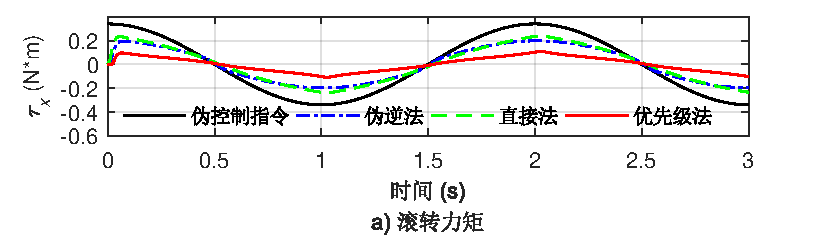
\includegraphics[scale=1]{Fig/Fig7a.pdf}
	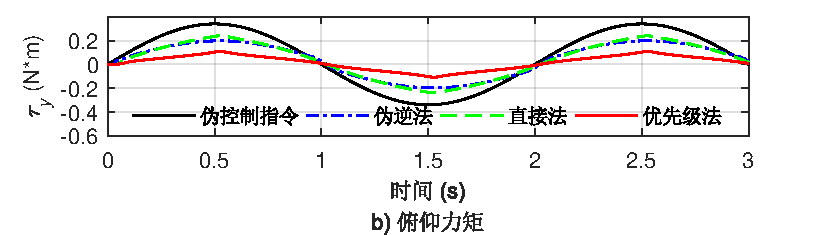
\includegraphics[scale=1]{Fig/Fig7b.pdf}
	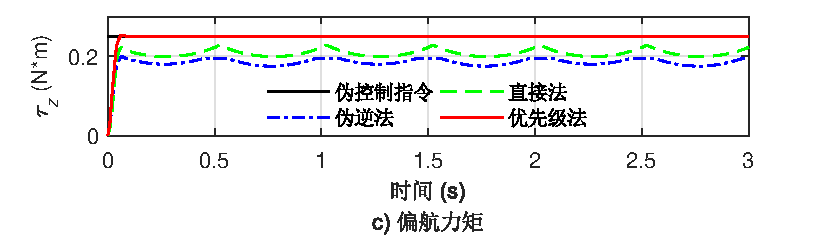
\includegraphics[scale=1]{Fig/Fig7c.pdf}
	\caption{\label{fig_Virtual_control_response}伪控制输入响应曲线}
\end{figure}

\section{双涵道仿真分析}
双涵道的控制分配中应用动态控制分配的优势主要体现在滚转通道上,因此在本节中,我们仅介绍滚转控制舵之一的$ \delta_3 $和操纵面$ \delta_9 $的对伪控制输入的响应情况,俯仰和偏航通道的伪控制输入保持为零, 采样周期为$\text{T}=0.01\,\text{s}$。 数字舵机和无刷直流电动机的动力学近似为一阶系统,假设和$ \delta_3 $和$ \delta_9 $相关的执行器的传递函数
\begin{align}
\dfrac{\delta_{ {3}}\left( s \right)}
{\delta_{c {3}}\left( s\right)}
=\dfrac{35}{s+35} \qquad
\dfrac{\delta_{ {9}}\left( s \right)}
{\delta_{c {9}}\left( s\right)}
=\dfrac{4}{s+4}
\end{align}
并设用做对比的静态控制分配器的参数为$ \bm{W}_1=\bm{I}_{9 \times 9}$,$\bm{W}_{2} = \bm{0}_{9 \times 9} $,$\bm{W}_v = \bm{I}_{3 \times 3}$,$ \gamma = 10^5 $和$ \bm{\delta}_s = \bm{0}_ {9 \times 1} $。 

动态控制分配器的参数取为
\begin{align}
\bm{S} = \left[ {\begin{array}{*{20}{c}}
	0&0&0&0&0&0&0&0&12.7591 \\ 
	0&{ - 0.0167}&0&{ 0.0167}&0&{ - 0.0167}&0&{ 0.0167}&0 \\ 
	0&{ - 0.0121}&0&{ 0.0269}&0&{ 0.0269}&0&{ - 0.0121}&0 
	\end{array}} \right]^\top
\end{align}
且$ \bm{W}_1 = \bm{I}_{9 \times 9}$,$\bm{W}_{2}={diag}(1,1,1,1,1,1,1,1,5)$,$ \bm{W}_v = \bm{I}_{3 \times 3} $和$\gamma =10^5$。

首先,系统在包含执行器动态补偿环节的情况下运行。当伪控制输入$ \bm{\tau} $(cmd)是阶跃信号时,两种分配方法的响应如图\ref {step}所示。开始时,所有操纵面一起移动。静态控制分配器(sca)在过渡过程中使涵道风扇转速差先增大后减小,动态控制分配器(dca)则使涵道风扇转速差缓慢增加。进入稳态后,sca使低效的的操纵面($ \delta_3 $)接近饱和,而dca仅使用高效的操纵面($ \delta_9 $),并避免$ \delta_3 $饱和。当伪控制输入是幅度为$6\,{\text{rad}}/{{{\text{s}}^{2}}}$且频率范围为$0.5 \sim 2\,\text{Hz}$的频率信号时,系统输出如图\ref{chirps}所示。dca根据带宽将伪控制输入分配给不同的执行器,将高频输入分配给高带宽执行器(数字舵机),将低频输入主要分配给低带宽执行器(电机)。而sca没有考虑执行器带宽的差异。
\begin{figure}[htbp]
	\centering	
	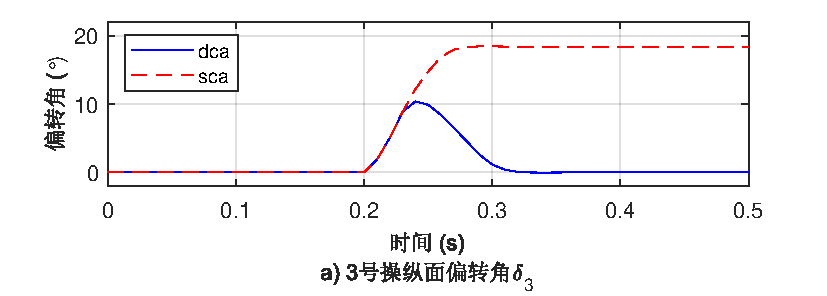
\includegraphics[scale=1]{Fig/TDF_step_response_a.pdf}
	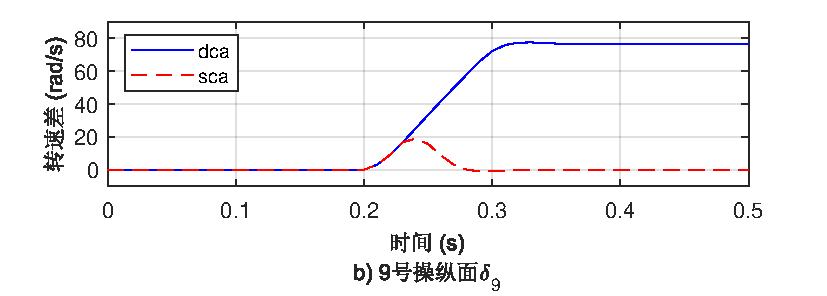
\includegraphics[scale=1]{Fig/TDF_step_response_b.pdf}
	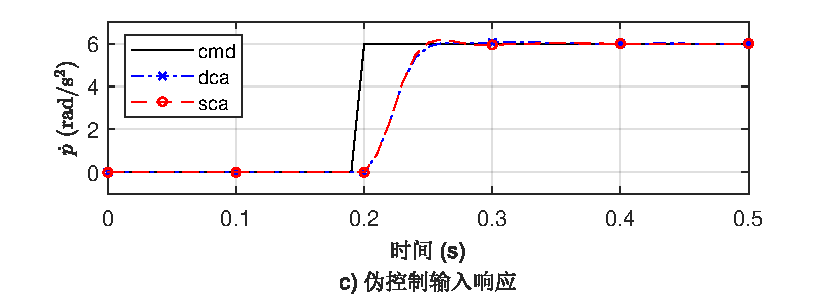
\includegraphics[scale=1]{Fig/TDF_step_response_c.pdf}
	\caption{\label{step}阶跃伪控制输入}
\end{figure}
%\begin{figure}[htbp]
%	\centering	
%%	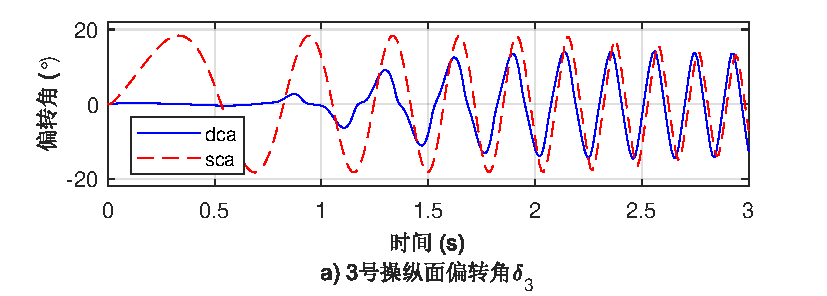
\includegraphics[scale=1]{Fig/TDF_chirps_response_a.pdf}
%%	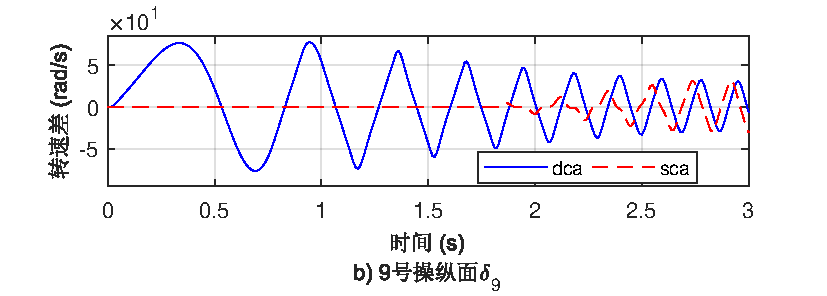
\includegraphics[scale=1]{Fig/TDF_chirps_response_b.pdf}
%\end{figure}
\begin{figure}[htbp]
	\centering	
	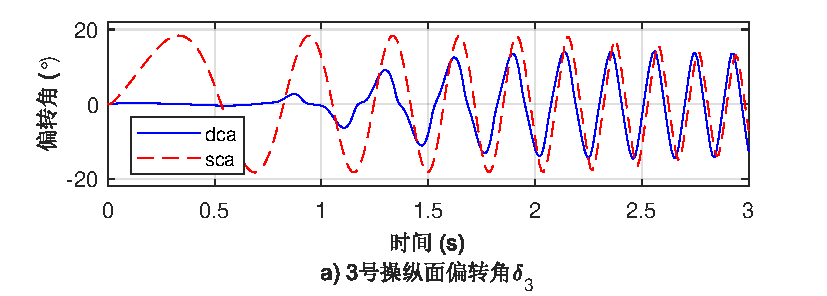
\includegraphics[scale=1]{Fig/TDF_chirps_response_a.pdf}
	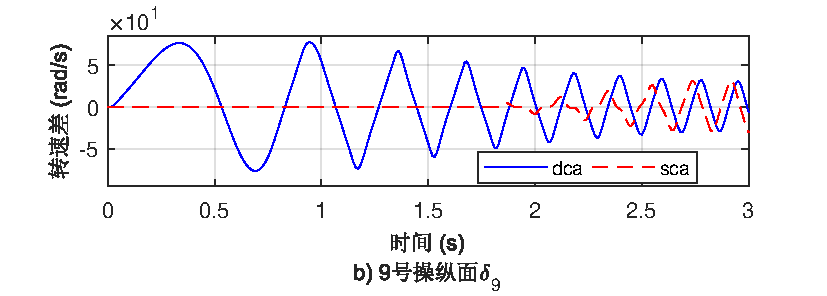
\includegraphics[scale=1]{Fig/TDF_chirps_response_b.pdf}
	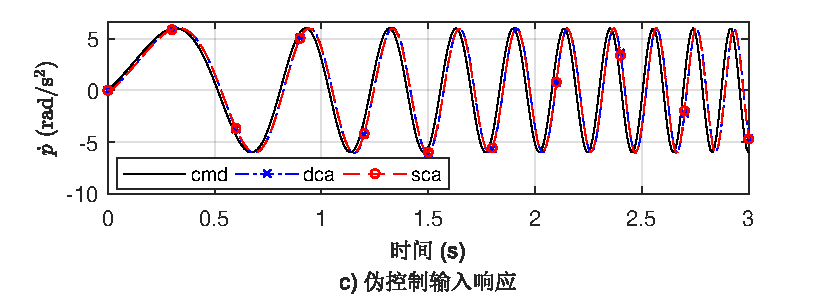
\includegraphics[scale=1]{Fig/TDF_chirps_response_c.pdf}
	\caption{\label{chirps}频率信号伪控制输入}
\end{figure}

然后,利用dca分配图\ref{chirps}中线性调频信号,对比系统在包含执行器补偿与否的两种情况的分配。 图\ref{compensation}显示了是否使用执行器补偿之间的区别。 当不使用补偿时,左右涵道风扇的实际转速差与给定的误差较大,这导致伪控制输入$ \bm {\tau} $和$ \bm {B \delta} $之间存在较大误差。 还可以看到,对于高带宽执行器,例如控舵$ \delta_3 $的执行器,忽略执行器动态并不会产生严重的不良影响,但是对于低带宽执行器,例如涵道风扇的执行器,执行器动态引起的衰减较明显。
\begin{figure}[htbp]
	\centering	
	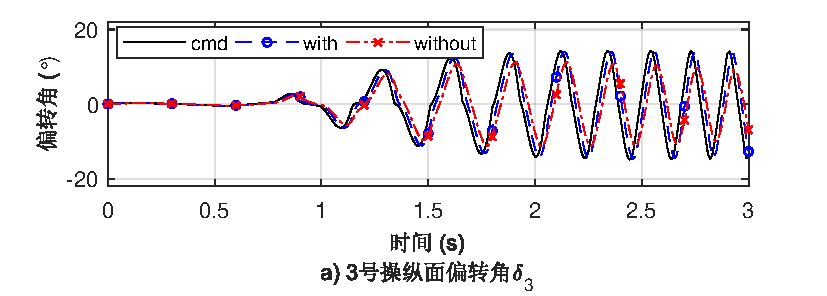
\includegraphics[scale=1]{Fig/TDF_chirps_without_comp_a.pdf}
	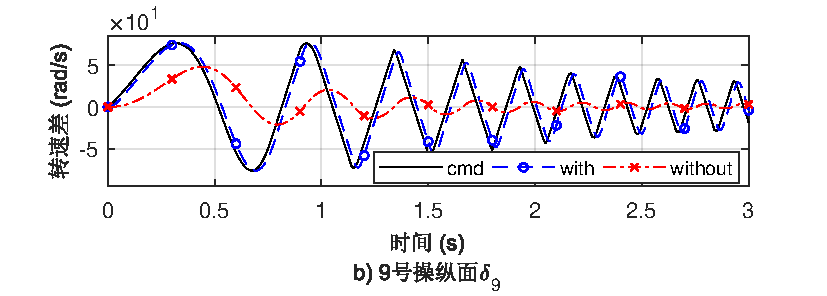
\includegraphics[scale=1]{Fig/TDF_chirps_without_comp_b.pdf}
	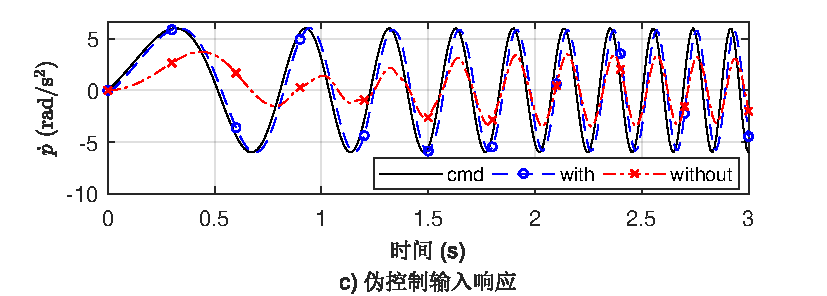
\includegraphics[scale=1]{Fig/TDF_chirps_without_comp_c.pdf}
	\caption{\label{compensation}含(with)与不含(without)执行器补偿的频率信号响应对比}
\end{figure}

从上述仿真结果可知,尽管不同分配方法对伪控制输入的响应几乎相同,但执行器的响应是不同的。 动态控制分配可以根据执行器带宽分配伪控制输入,并减少操纵面饱和的几率,并间接减小双涵道控制舵的气动阻力。 此外,对分配器输出指令的补偿有效地减少了由执行器动力学引起的不良影响,最终减小了分配误差。
%
\section{飞行试验}
%\subsection{分配算法对比}
%利用所设计的ADRC控制以及分配算法进行飞行试验,抗干扰效果以及控制分配的具体情况也将在下文展示。
%,其中扰动观测器ESO的输出$\bm{z}_1$、$\bm{z}_2$、$\bm{z}_3$分别表示估计的欧拉角、欧拉角的导数、系统总和扰动。TD的输出$\bm{v}_1$、$\bm{v}_2$表示给定欧拉角$[\varphi_c \quad \theta_c \quad \psi_c]^\top$的过渡过程及其微分信号。
在图\ref{fig_flight}所示的涵道风扇式无人机上做不同分配算法的对照试验,无人机参数如表1所示,试验时应用ADRC进行姿态控制,控制律为如式\eqref{control_law}所示,闭环系统如图\ref{fig_flight_control_system}所示。$\bm{I}\bm{z}_3$即估计的扰动力矩,扰动补偿为$\bm{\tau}_1=-\bm{I}\bm{z}_3$。每个通道的NLSEF类似地由式\eqref{NLSEF}给出,总的NLSEF的输出为$\bm{\tau}_2=\bm{u}_0$。试验中除控制分配算法不同外,控制律、参考指令、飞行环境均相同。系统控制周期$T=0.01s$,在定高且锁尾模式下飞行。
\begin{figure}[htbp]
	\centering	
	\includegraphics[scale=1]{Fig/Fig8b.jpg}
	\caption{\label{fig_flight}飞行试验}
\end{figure}
\begin{figure}[htbp]
	\centering	
	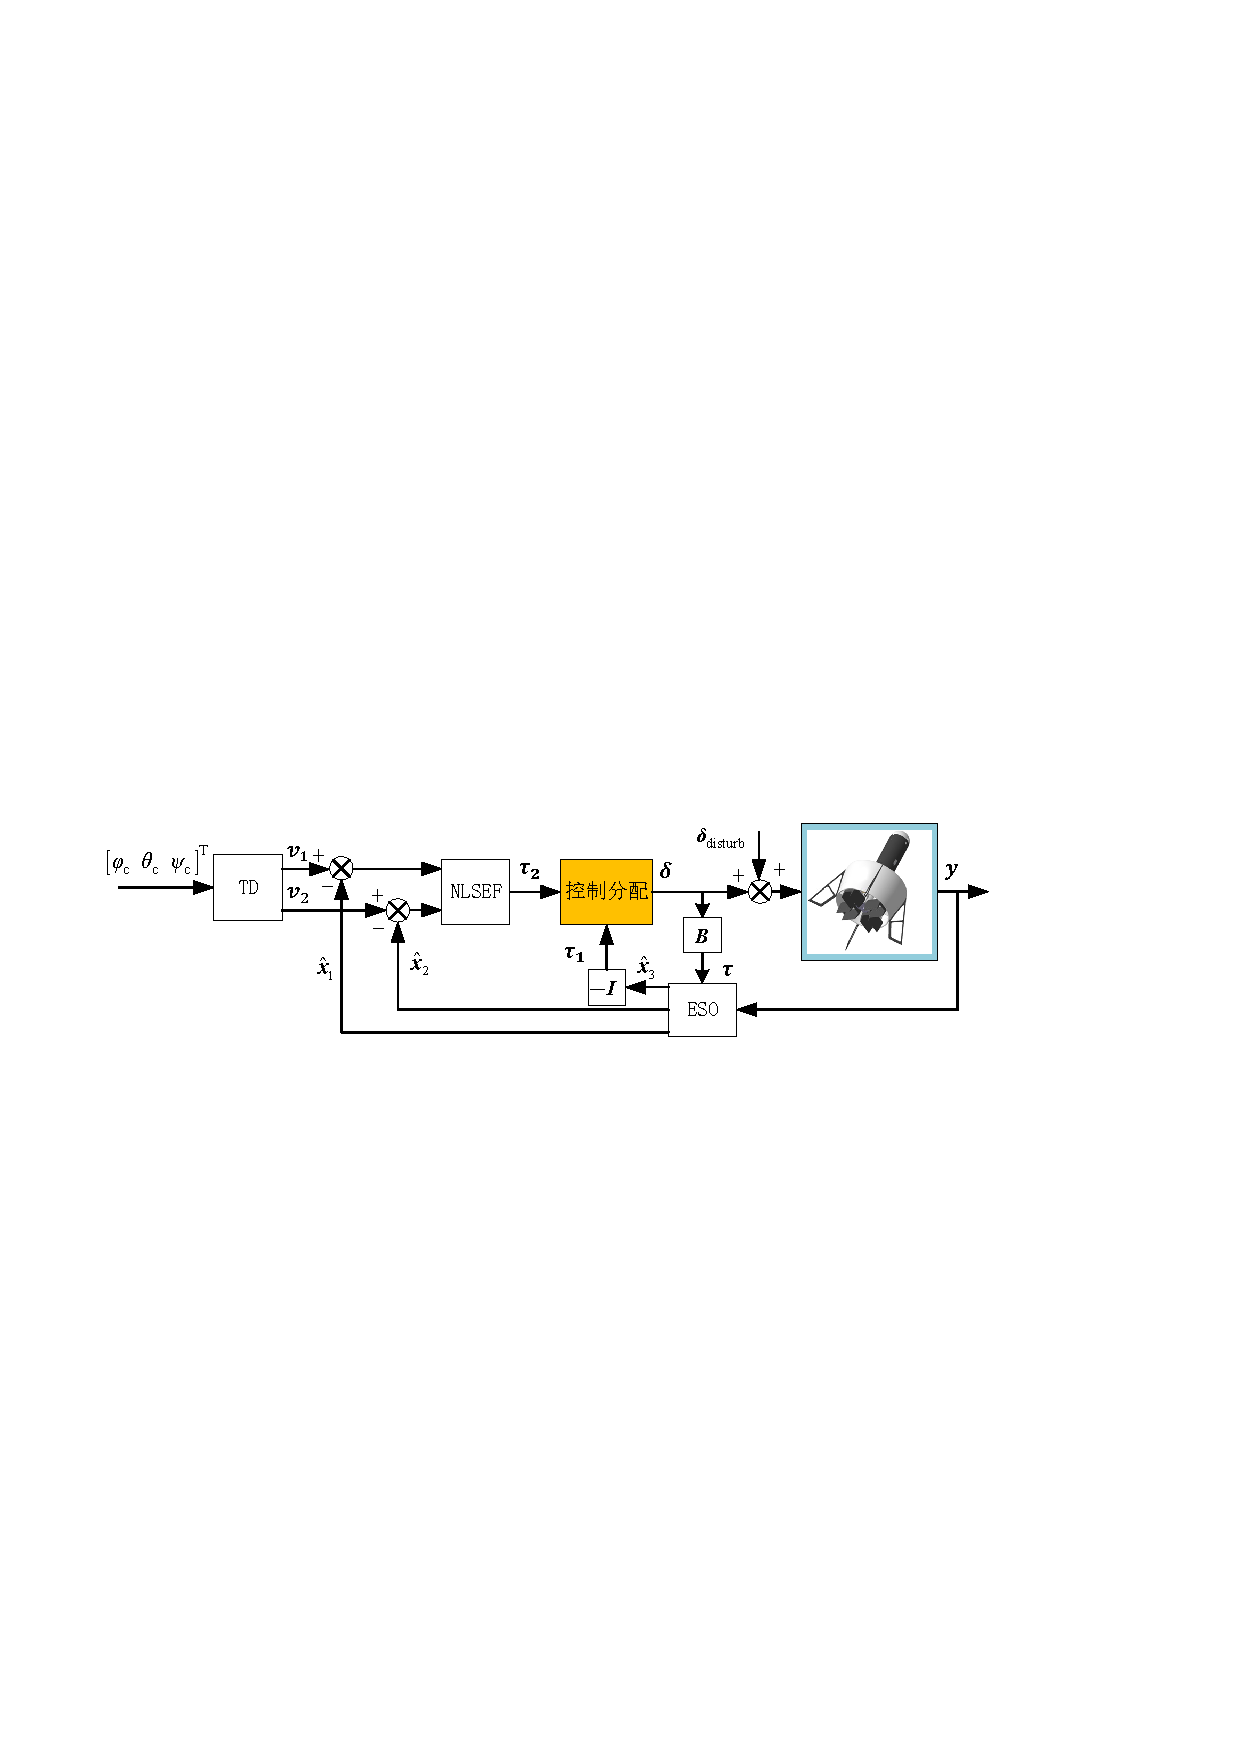
\includegraphics[scale=0.9]{Fig/Fig9.pdf}
	\caption{\label{fig_flight_control_system}飞控系统框图}
\end{figure}

将$\bm{\tau}_1$设为最高优先级,$\bm{\tau}_2$设为低优先级。操纵面物理约束如式\eqref{position_constraints}所示,为方便后续试验中添加$9{}^\circ $的操纵面扰动,试验时在控制程序中统一设定操纵面最大偏转角为$11{}^\circ $。如前文所述,忽略执行器动力学,舵面偏转角用其执行器的指令$\bm{\delta} $近似。姿态角参考输入为滚转、俯仰通道$20{}^\circ $的阶跃信号,航向角保持起飞时锁定的角度,统一为正北方向(零度偏航角)。
\subsection{无外扰的姿态跟踪}
若不添加扰动,分别使用伪逆法、直接分配法、优先级法进行控制分配,姿态角的阶跃响应曲线如图\ref{fig_step_without_d}所示,相应的操纵面偏转角响应曲线如图\ref{fig_Deflection_angle_without_d}所示。由图\ref{fig_step_without_d}可知三种方法下的阶跃响应性能指标比较接近。比较三种方法的操纵面曲线,可知品质因数较小的伪逆法更容易饱和,而直接分配法和优先级分配法由于其可达集是整个AMS边界所包围的力矩空间,因而操纵面饱和的时间相对较短。
\begin{figure}[htbp]
	\centering	
	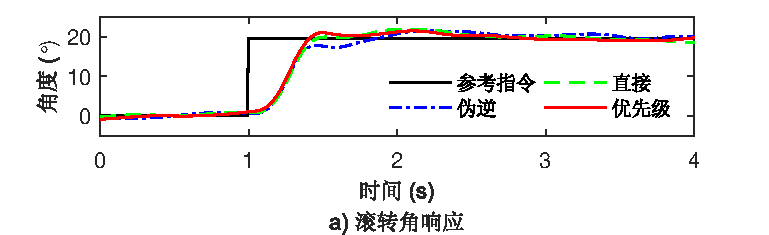
\includegraphics[scale=1]{Fig/Fig10a.pdf}
%	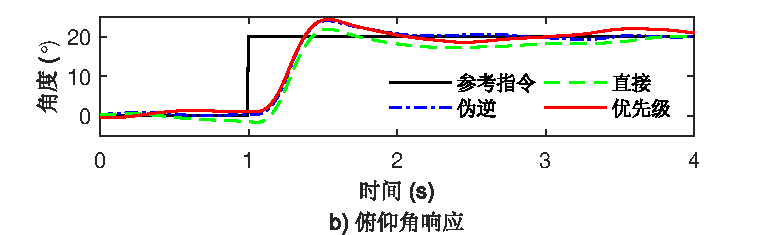
\includegraphics[scale=1]{Fig/Fig10b.pdf}
\end{figure}
\begin{figure}[htbp]
	\centering	
%			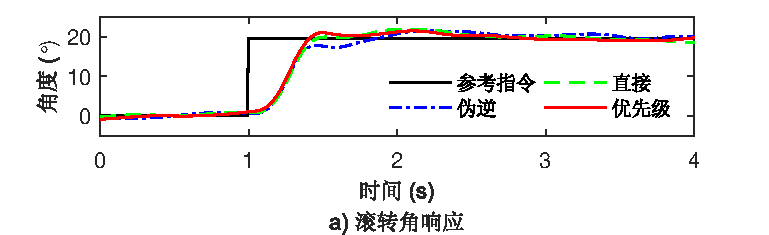
\includegraphics[scale=1]{Fig/Fig10a.pdf}
			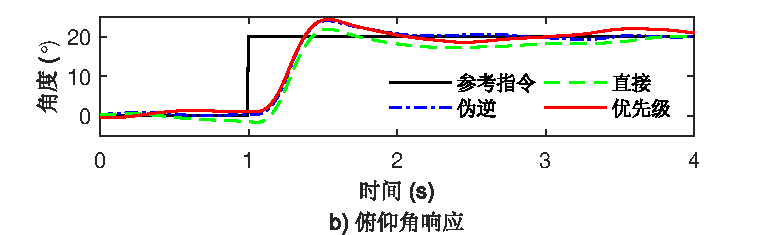
\includegraphics[scale=1]{Fig/Fig10b.pdf}
	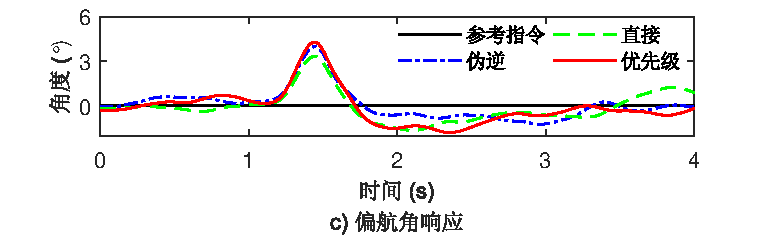
\includegraphics[scale=1]{Fig/Fig10c.pdf}
	\caption{\label{fig_step_without_d}在无外扰的情况下,分别使用伪逆、直接、优先级分配的阶跃响应}
\end{figure}	
\begin{figure}[htbp]
	\centering	
	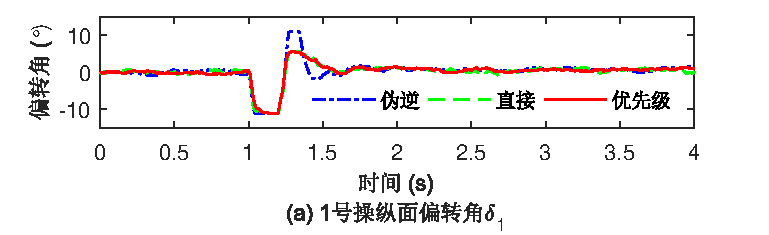
\includegraphics[scale=1]{Fig/Fig11a.pdf}
	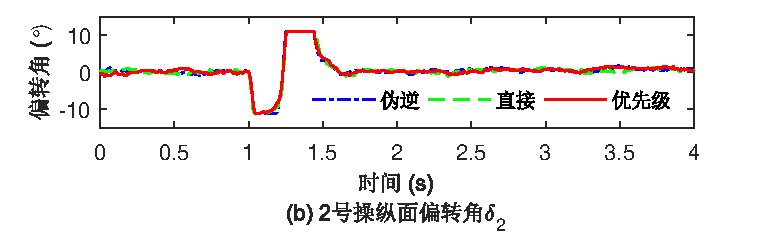
\includegraphics[scale=1]{Fig/Fig11b.pdf}
	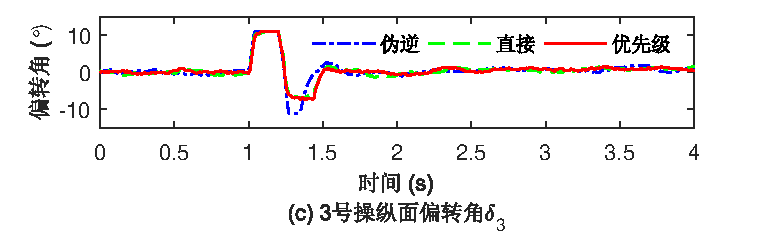
\includegraphics[scale=1]{Fig/Fig11c.pdf}
\end{figure}
\begin{figure}[htbp]
	\centering	
%	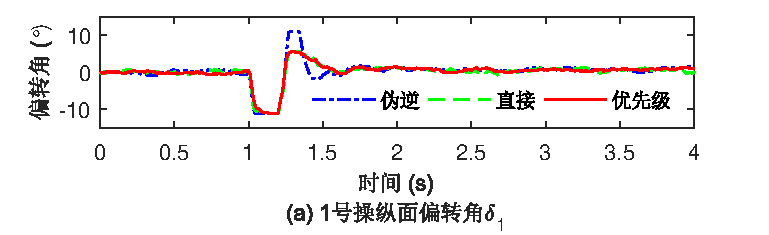
\includegraphics[scale=1]{Fig/Fig11a.pdf}
%	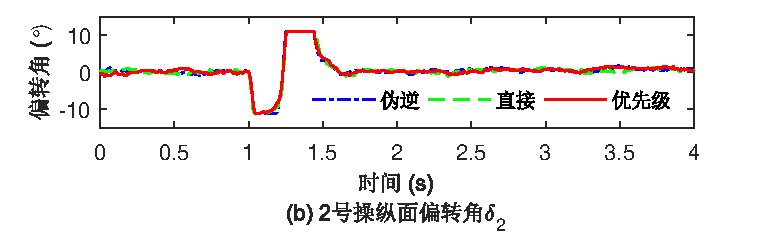
\includegraphics[scale=1]{Fig/Fig11b.pdf}
%	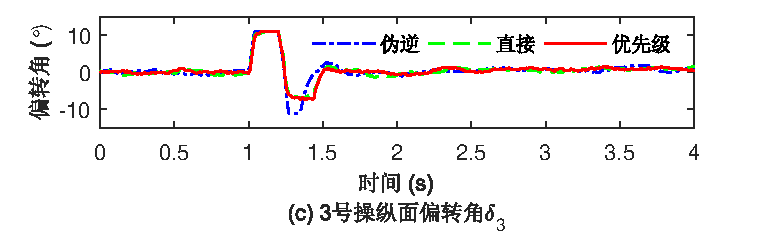
\includegraphics[scale=1]{Fig/Fig11c.pdf}
	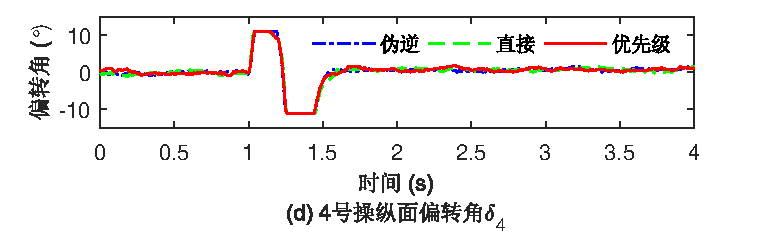
\includegraphics[scale=1]{Fig/Fig11d.pdf}
	\caption{\label{fig_Deflection_angle_without_d}无外扰时的1到4号舵面偏转角}
\end{figure}
\subsection{常值扰动下的姿态跟踪}
若添加恒定扰动$\bm{\delta }_{disturb}= [9{}^\circ \quad 9{}^\circ \quad 9{}^\circ \quad 9{}^\circ]^\top $到操纵面,用于产生偏航通道的扰动力矩,ESO的输出$\bm{\tau}_1$将主要用于补偿该力矩。待系统进入稳态后开始计时,姿态角参考输入同上文。伪逆法和直接分配法的姿态角响应曲线如图\ref{fig_id_step_with_d}所示,优先级分配法的姿态角响应曲线如图\ref{fig_p_step_with_d}所示,三种方法相应的操纵面偏转角响应曲线如图\ref{fig_Deflection_angle_with_d}所示。

由图\ref{fig_id_step_with_d}可知伪逆法和直接分配法都在输入参考指令后航向角由于扰动的影响持续减小,最终使系统发散,3秒后已经由回收设备介入。而由图\ref{fig_p_step_with_d}可知优先级分配法使系统仍稳定跟踪参考输入,和图\ref{fig_step_without_d}的结果相比仅响应速度变慢。由图\ref{fig_Deflection_angle_with_d}可知,系统在阶跃信号到来之前,操纵面偏转角稳定在$\bm{\delta }_{disturb}$附近,表明$\bm{\tau}_1$是可达的。在第1秒到第1.5秒的瞬态响应期间,操纵面饱和即表明参考指令使得误差反馈输出的$\bm{\tau}_2$叠加$\bm{\tau}_1$的结果$\bm{\tau}_1+\bm{\tau}_2$不可达。在优先级分配法中,$\bm{\tau}_1$被设置为高优先级,使操纵面仅在补偿扰动所需的偏转角附近动作,保证高优先级分量尽可能的得到执行,因此始终能抵抗扰动的影响。而伪逆法和直接分配法都由于误差反馈的影响,操纵面在其约束范围内动作,高优先级分量的执行得不到保证,最终导致输出耦合,表现为输入阶跃参考指令后系统发散。
\begin{figure}[htbp]
	\centering	
	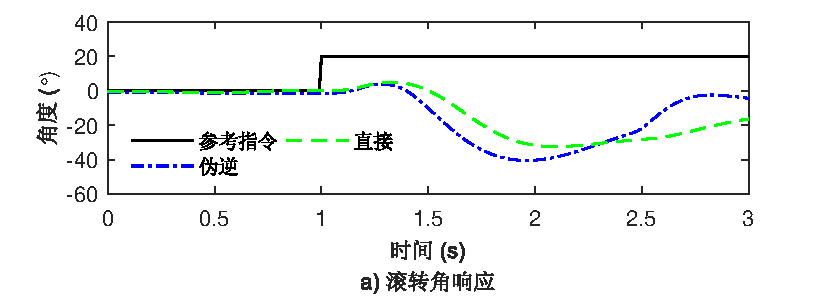
\includegraphics[scale=1]{Fig/Fig12a.pdf}
	%	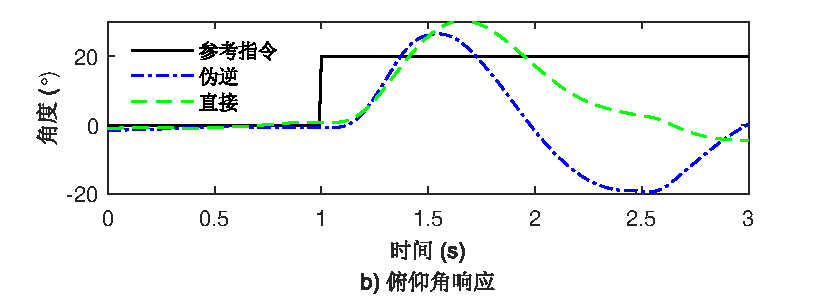
\includegraphics[scale=1]{Fig/Fig12b.pdf}
\end{figure}
\begin{figure}[htbp]
	\centering	
%		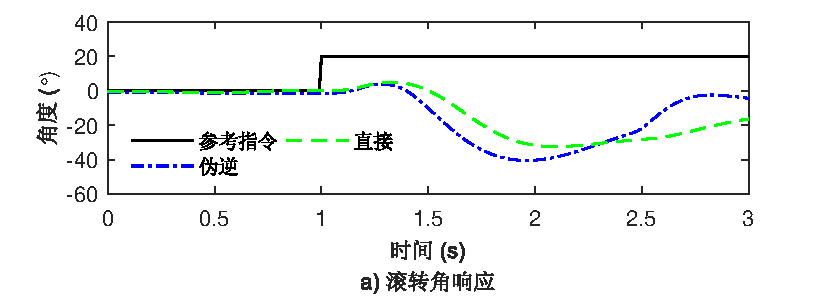
\includegraphics[scale=1]{Fig/Fig12a.pdf}
	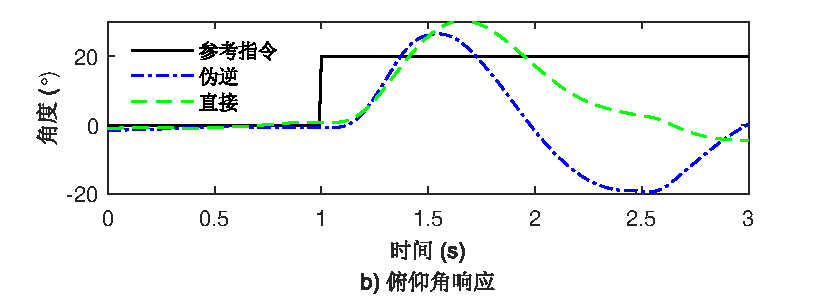
\includegraphics[scale=1]{Fig/Fig12b.pdf}
	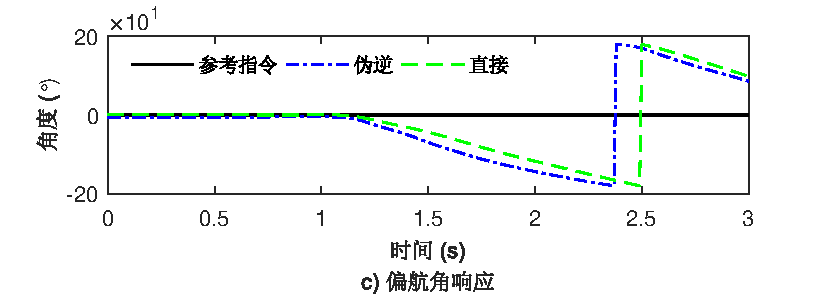
\includegraphics[scale=1]{Fig/Fig12c.pdf}
	\caption{\label{fig_id_step_with_d}添加扰动,分别使用伪逆、直接分配的阶跃响应}
	%	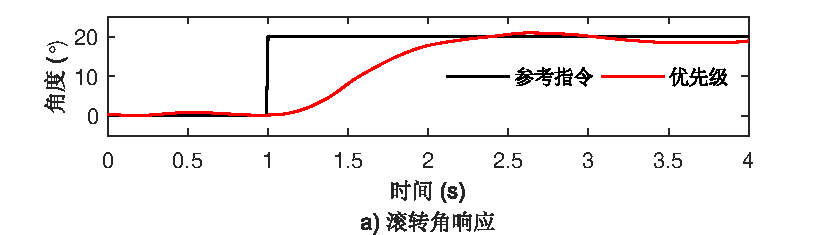
\includegraphics[scale=1]{Fig/Fig13a.pdf}
	%	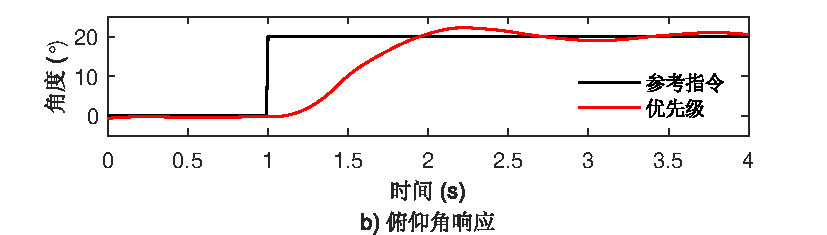
\includegraphics[scale=1]{Fig/Fig13b.pdf}
\end{figure}
\begin{figure}[htbp]
	\centering	
	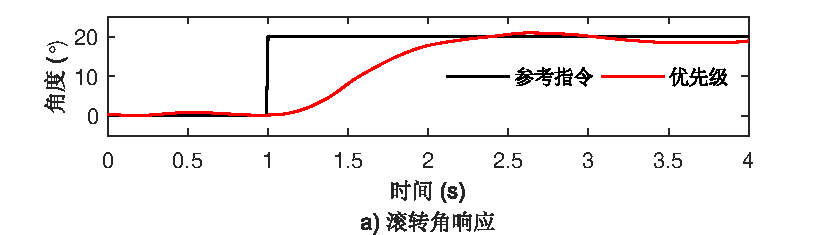
\includegraphics[scale=1]{Fig/Fig13a.pdf}
	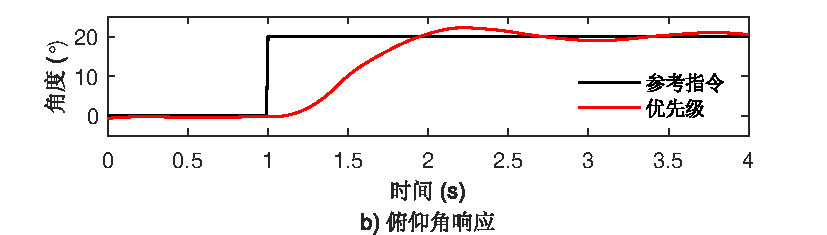
\includegraphics[scale=1]{Fig/Fig13b.pdf}
	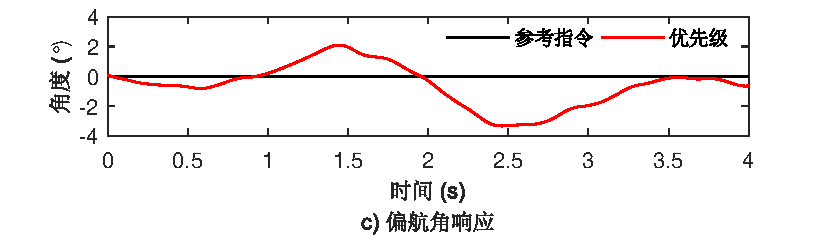
\includegraphics[scale=1]{Fig/Fig13c.pdf}
	\caption{\label{fig_p_step_with_d}添加扰动,使用优先级分配的阶跃响应}
\end{figure}
\begin{figure}[htbp]
	\centering	
	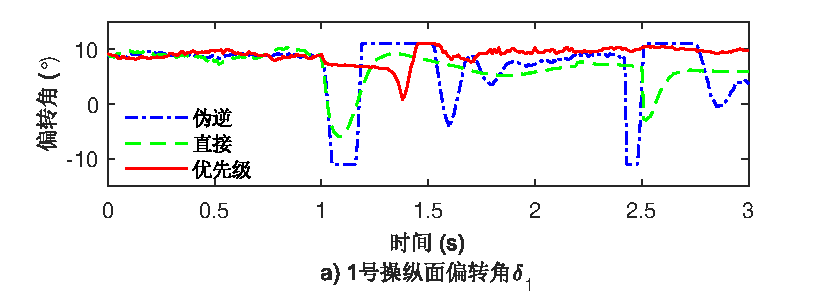
\includegraphics[scale=1]{Fig/Fig14a.pdf}
	\includegraphics[scale=1]{Fig/Fig14b.pdf}
	\includegraphics[scale=1]{Fig/Fig14c.pdf}
%\end{figure}
%\begin{figure}[htbp]
%	\centering	
	\includegraphics[scale=1]{Fig/Fig14d.pdf}
	\caption{\label{fig_Deflection_angle_with_d}添加扰动时的1到4号舵面偏转角}
\end{figure}
\subsection{正弦扰动抑制效果}
对比ADRC和PID控制器的扰动抑制能力。当使用ADRC控制时,闭环系统仍如图\ref{fig_flight_control_system}所示。当使用PID控制器时,控制分配算法不变,但实际上以及退化为直接分配法,闭环系统如图\ref{allo_base_PID}所示。给定姿态角为$[\varphi_c \quad \theta_c \quad \psi_c]^\top=[0 \quad 0 \quad 0]^\top$,并且添加扰动$\bm{\delta }_{disturb}= [0.34sin(0.1\pi t) \quad 0 \quad 0.34sin(0.1\pi t) \quad 0]^\top $。ADRC和PID控制下的滚转角响应如图\ref{PID_ADRC}所示。
\begin{figure}[htbp]
	\centering	
	\includegraphics[scale=1]{Fig/allo_base_PID.pdf}
	\caption{\label{allo_base_PID}正弦扰动抑制试验闭环系统}
\end{figure}
\begin{figure}[htbp]
	\centering	
%	\includegraphics[scale=0.7]{Fig/ADRC_r.png}
	\includegraphics[scale=1]{Fig/PID_ADRC.pdf}
	\caption{\label{PID_ADRC}正弦扰动抑制效果}
\end{figure}
\section{本章小结}
本章是对前几章的内容进行的仿真及试验验证。

在仿真分析中,分别对单涵道和双涵道进行了分析。在单涵道仿真中,先利用角速度环闭环控制验证了第二章所建立的模型的准确性,接着利用利用ADRC控制姿态,观察ESO估计的扰动与系统的真实扰动的接近程度,证实了所设计的ESO的收敛性。最后仿真验证了优先级分配方法对高优先级分量的跟踪效果优于传统算法。在双涵道仿真中,我们的重点是讨论控制分配。分别讨论了伪控制输入为阶跃信号和调频信号时,动态控制分配的分配效果。仿真结果表明,带执行器动态补偿的动态控制分配方法可以防止高带宽执行器提前饱和,伪控制输入可以有效地分配给不同带宽的执行器。

%在飞行试验中,首先在没有外部扰动的情况下,对比了不同分配算法下的操纵面偏转角曲线以及姿态跟踪曲线。伪逆法更容易饱和这一事实,证实了在上一章中得出的其可达集小的结论。其次在常值扰动下,对比姿态跟踪曲线以及操纵面偏转角曲线,证实了优先级分配法可以最大限度保持输出解耦,相当于提高了稳定性。最后我们人为添加一个正弦扰动,结果表明所设计的ADRC控制律比常规的PID控制有更好的扰动抑制能力。

在飞行试验中,以单涵道为例,将本文所提出的优先级方法的应用于的其控制分配中。该试验中,将控制律分解为两部分:一部分与系统抗扰动能力相关,作为高优先级分量;另一部分与瞬态响应相关,作为低优先级分量。试验结果表明,优先级分配法能保证可达的高优先级分量无误差分配,系统保持一定的输出解耦,而传统分配方法则因为执行器饱和而导致输出耦合。最后考察了正弦扰动下的扰动抑制能力,结果表明所设计的ADRC控制律比常规的PID控制有更好的扰动抑制能力。




